\documentclass[11pt,a4paper]{article}

% --- Packages ---
\usepackage[utf8]{inputenc}
\usepackage[margin=0.72in,headheight=14.5pt]{geometry}
\usepackage{fancyhdr}
\usepackage{amsmath,amssymb}
\usepackage{booktabs}
\usepackage{tabularx}
\usepackage{multirow}
\usepackage{ragged2e}
\usepackage{listings}
\usepackage{xcolor}
\usepackage{graphicx}
\usepackage{hyperref}
\usepackage{caption}
\usepackage{subcaption}
\usepackage{float}
\usepackage{microtype}
\usepackage{enumitem}

% Prevent vertical stretching and minimize gaps around floats/lists
\raggedbottom
\setlist{itemsep=1pt, topsep=2pt, parsep=0.5pt, partopsep=0pt}
\setlength{\intextsep}{5pt plus 1pt minus 1pt}
\setlength{\textfloatsep}{5pt plus 1pt minus 1pt}
\setlength{\abovecaptionskip}{3pt}
\setlength{\belowcaptionskip}{2pt}
\setlength{\abovedisplayskip}{3pt plus 1pt minus 1pt}
\setlength{\belowdisplayskip}{3pt plus 1pt minus 1pt}

% Float placement tolerances
\renewcommand{\topfraction}{0.95}
\renewcommand{\bottomfraction}{0.95}
\renewcommand{\textfraction}{0.05}
\renewcommand{\floatpagefraction}{0.85}

% Section spacing
\makeatletter
\renewcommand\section{\@startsection {section}{1}{\z@}%
  {-2.0ex \@plus -0.5ex \@minus -.2ex}%
  {1.0ex \@plus .2ex}%
  {\normalfont\Large\bfseries}}
\renewcommand\subsection{\@startsection{subsection}{2}{\z@}%
  {-1.5ex\@plus -0.4ex \@minus -.2ex}%
  {0.6ex \@plus .2ex}%
  {\normalfont\large\bfseries}}
\renewcommand\subsubsection{\@startsection{subsubsection}{3}{\z@}%
  {-1.2ex\@plus -0.3ex \@minus -.1ex}%
  {0.4ex \@plus .1ex}%
  {\normalfont\normalsize\bfseries}}
\makeatother

% --- Hyperref Setup ---
\hypersetup{
  colorlinks=true,
  linkcolor=blue!70!black,
  citecolor=blue!70!black,
  urlcolor=blue!70!black
}

% --- Header and Footer ---
\pagestyle{fancy}
\fancyhf{}
\lhead{CISCO Packet Tracer Network Experiments}
\rhead{Computer Networks Lab: Assignment 6}
\cfoot{Page \thepage}
\renewcommand{\headrulewidth}{0.4pt}
\renewcommand{\footrulewidth}{0.0pt}

% --- Code Listing Styling ---
\definecolor{codegreen}{rgb}{0,0.6,0}
\definecolor{codegray}{rgb}{0.45,0.45,0.45}
\definecolor{codepurple}{rgb}{0.58,0,0.82}
\definecolor{backcolour}{rgb}{0.96,0.97,0.98}
\definecolor{keycolor}{rgb}{0.0,0.2,0.6}

\lstdefinestyle{cmdstyle}{
  backgroundcolor=\color{backcolour},
  basicstyle=\ttfamily\small,
  columns=flexible,
  numbers=none,
  frame=single,
  rulecolor=\color{black!20},
  breaklines=true,
  keepspaces=true,
  aboveskip=3pt,
  belowskip=3pt
}

\begin{document}

% =========================================================================
% COVER PAGE
% =========================================================================
\hypersetup{pageanchor=false}
\begin{titlepage}
  \centering
  \vspace*{1.2cm}
  {\Large \textbf{JADAVPUR UNIVERSITY}}\\[0.3cm]
  {\large DEPARTMENT OF COMPUTER SCIENCE AND ENGINEERING}\\[1.8cm]

  \rule{\linewidth}{1.2pt}\\[0.4cm]
  {\huge \textbf{Assignment 6 Report}}\\[0.3cm]
  {\LARGE \textbf{CISCO Packet Tracer Network Experiments}}\\[0.3cm]
  {\large \textit{LAN Construction with Hubs and Switches, Inter-LAN Routing, DHCP Configuration, DNS and Server Services}}\\[0.3cm]
  \rule{\linewidth}{1.2pt}\\[1.8cm]

  \begin{minipage}[t]{0.88\textwidth}
    \large
    \textbf{Course:} Computer Networks Laboratory (BCSE-III)\\[0.25cm]
    \textbf{Student Name:} Mandeep Shaw\\[0.25cm]
    \textbf{Section:} A1\\[0.25cm]
    \textbf{Roll Number:} 302510501002\\[0.25cm]
    \textbf{Assignment:} Assignment 6 (CISCO Packet Tracer Network Experiments)\\[0.25cm]
    \textbf{Date of Submission:} November 2026
  \end{minipage}

  \vfill
  {\small Faculty of Engineering and Technology $\bullet$ Jadavpur University, Kolkata, India}
  \vspace*{0.8cm}
\end{titlepage}

% =========================================================================
% TABLE OF CONTENTS
% =========================================================================
\hypersetup{pageanchor=true}
\pagenumbering{roman}
\tableofcontents
\newpage
\pagenumbering{arabic}
\setcounter{page}{1}

% =========================================================================
% SECTION 1: OVERVIEW AND OBJECTIVES
% =========================================================================
\section{Overview and Objectives}
Cisco Packet Tracer is a comprehensive network simulation and visualization tool developed by Cisco Systems that allows students to design, build, configure, and troubleshoot virtual networks without requiring physical hardware. It supports a wide range of Cisco devices including routers, switches, hubs, and end-host PCs, providing a realistic environment for experimenting with network topologies, IP addressing, routing protocols, and network services.

This assignment explores fundamental networking concepts through seven progressive experiments in Cisco Packet Tracer, covering Layer-2 LAN construction, address resolution, inter-network routing with static routes, and application-layer services (DHCP, DNS, HTTP, FTP).

\subsection{Objectives}
The primary objectives of this laboratory assignment are:
\begin{itemize}
  \item Establish direct point-to-point connectivity between two hosts using a crossover cable and verify reachability via ICMP ping.
  \item Construct a Local Area Network (LAN) using a hub and verify broadcast-domain connectivity between all host pairs.
  \item Construct a LAN using a Layer-2 switch and observe the dynamic learning behavior of MAC address tables and ARP caches.
  \item Interconnect hub-based and switch-based LANs via a crossover cable and verify cross-LAN reachability.
  \item Design and configure a multi-LAN internetwork with two Cisco 1841 routers, static routing, and WAN serial links to enable inter-LAN communication across different IP subnets.
  \item Configure DHCP servers on individual LANs to dynamically assign IP addresses and default gateways to hosts.
  \item Deploy a complete LAN with web, FTP, DHCP, and DNS servers, configure DNS records, and verify name-based service access.
\end{itemize}

% =========================================================================
% SECTION 2: QUESTION 1 - CROSSOVER CABLE
% =========================================================================
\section{Question 1: Direct Host-to-Host Connection via Crossover Cable}

\subsection{Problem Statement}
\begin{quote}
\small\textit{Connect two hosts back-to-back with a crossover cable. Assign IP addresses, and see whether they are able to ping each other.}
\end{quote}

\subsection{Experimental Setup}
Two PCs (PC0 and PC1) were placed in the Cisco Packet Tracer workspace and connected directly using a \textbf{crossover Ethernet cable}. A crossover cable is required for direct host-to-host connections because both devices are DTE (Data Terminal Equipment) devices that transmit on the same pin pairs. The crossover cable swaps the transmit and receive pairs (pins 1,2 $\leftrightarrow$ pins 3,6), enabling proper communication.

\subsubsection{IP Address Configuration}
\begin{table}[H]
  \centering
  \begin{tabular}{lccc}
    \toprule
    \textbf{Host} & \textbf{IP Address} & \textbf{Subnet Mask} & \textbf{Interface} \\
    \midrule
    PC0 & \texttt{192.168.1.1} & \texttt{255.255.255.0} & FastEthernet0 \\
    PC1 & \texttt{192.168.1.2} & \texttt{255.255.255.0} & FastEthernet0 \\
    \bottomrule
  \end{tabular}
  \caption{IP address assignment for direct host-to-host connection.}
  \label{tab:q1_ip}
\end{table}

\subsection{Ping Test Results}
The connectivity was verified by issuing ping commands from PC0 to PC1 and vice versa.

\begin{figure}[H]
  \centering
  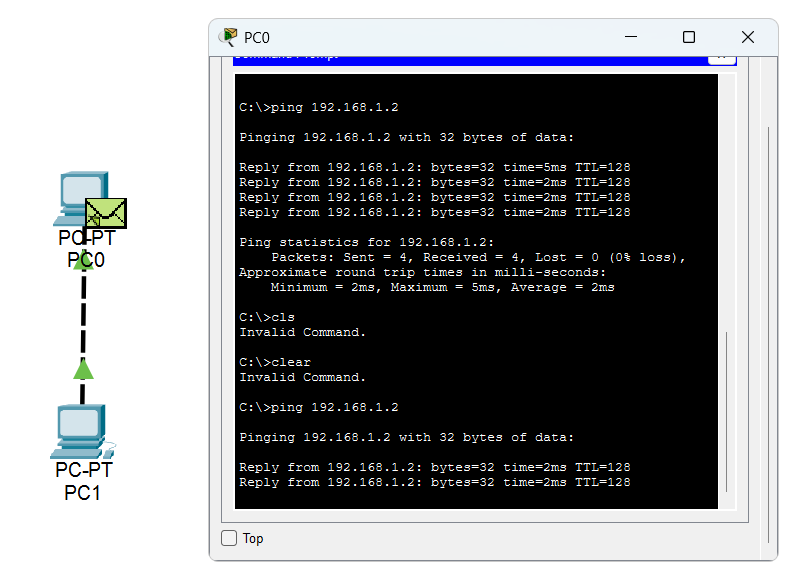
\includegraphics[width=1.0\textwidth]{Q1.png}
  \caption{Cisco Packet Tracer showing two PCs connected via crossover cable. PC0 successfully pings PC1 (\texttt{192.168.1.2}) with 0\% packet loss.}
  \label{fig:q1_ping}
\end{figure}

As shown in Figure \ref{fig:q1_ping}:
\begin{itemize}
  \item \textbf{From PC0:} \texttt{ping 192.168.1.2} --- All 4 packets received successfully (0\% loss). The first ping had a slightly higher latency (5ms) due to the initial ARP resolution, while subsequent pings completed in 2ms.
  \item \textbf{From PC1 (second ping from PC0):} The second ping session also shows all replies received with 2ms round-trip time, confirming stable bidirectional connectivity.
\end{itemize}

\noindent \textbf{Conclusion:} Two hosts connected back-to-back with a crossover cable can successfully communicate when assigned IP addresses on the same subnet. The crossover cable eliminates the need for intermediate networking equipment (hub or switch).

% =========================================================================
% SECTION 3: QUESTION 2 - LAN WITH HUB
% =========================================================================
\section{Question 2: LAN-A with Three Hosts Using a Hub}

\subsection{Problem Statement}
\begin{quote}
\small\textit{Create a LAN (named LAN-A) with 3 hosts using a hub. Ping each pair of nodes.}
\end{quote}

\subsection{Experimental Setup}
Three PCs (PC0(1), PC1(1), PC2) were connected to a central \textbf{Hub-PT (Hub0)} using straight-through Ethernet cables. A hub is a Layer-1 (Physical Layer) device that operates by broadcasting all incoming frames to every connected port, creating a single collision domain.

\subsubsection{IP Address Configuration}
\begin{table}[H]
  \centering
  \begin{tabular}{lccc}
    \toprule
    \textbf{Host} & \textbf{IP Address} & \textbf{Subnet Mask} & \textbf{Network} \\
    \midrule
    PC0(1) & \texttt{192.168.2.1} & \texttt{255.255.255.0} & LAN-A \\
    PC1(1) & \texttt{192.168.2.2} & \texttt{255.255.255.0} & LAN-A \\
    PC2    & \texttt{192.168.2.3} & \texttt{255.255.255.0} & LAN-A \\
    \bottomrule
  \end{tabular}
  \caption{IP address assignment for LAN-A (hub-based network).}
  \label{tab:q2_ip}
\end{table}

\subsection{Ping Test Results}
From the Command Prompt on PC0(1), ping tests were conducted to both PC1(1) and PC2:

\begin{figure}[H]
  \centering
  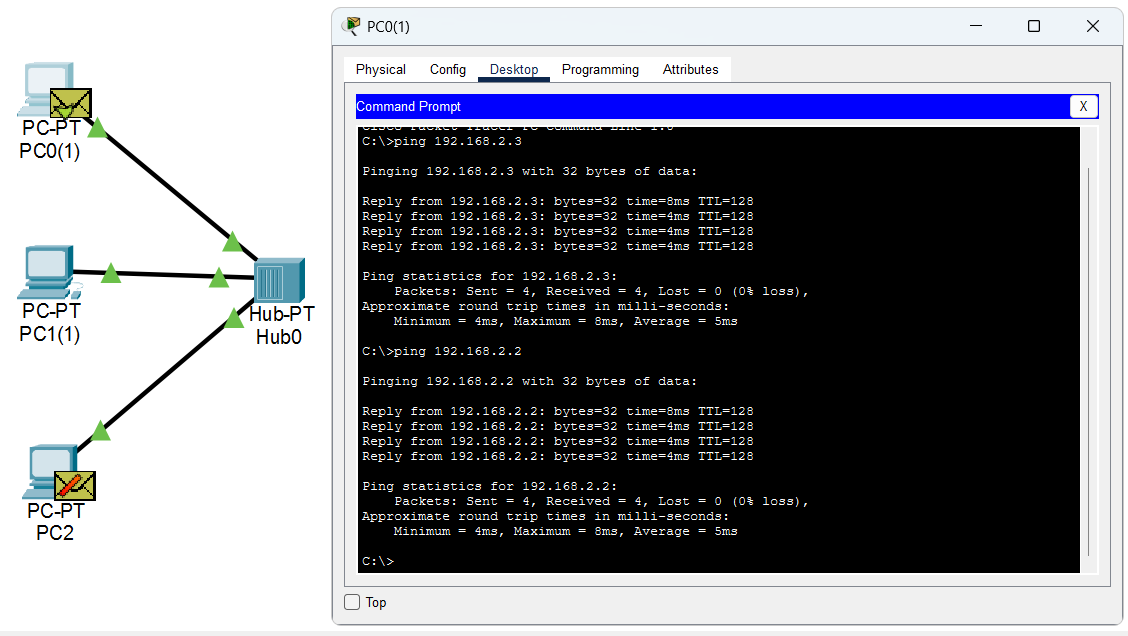
\includegraphics[width=17cm, height=12cm]{Q2.png}
  \caption{LAN-A topology with three hosts connected via Hub0. PC0(1) successfully pings \texttt{192.168.2.3} (PC2) and \texttt{192.168.2.2} (PC1(1)) with 0\% packet loss.}
  \label{fig:q2_ping}
\end{figure}

As shown in Figure \ref{fig:q2_ping}:
\begin{itemize}
  \item \texttt{ping 192.168.2.3} (PC2): 4/4 packets received, Min=4ms, Max=8ms, Avg=5ms.
  \item \texttt{ping 192.168.2.2} (PC1(1)): 4/4 packets received, Min=4ms, Max=8ms, Avg=5ms.
\end{itemize}

\noindent \textbf{Observation:} All three hosts in LAN-A can communicate with each other through the hub. The hub broadcasts every frame to all ports, so all hosts receive all traffic regardless of the intended destination. This creates a single collision domain but allows connectivity among all connected devices.

% =========================================================================
% SECTION 4: QUESTION 3 - LAN WITH SWITCH
% =========================================================================
\section{Question 3: LAN-B with Three Hosts Using a Switch}

\subsection{Problem Statement}
\begin{quote}
\small\textit{Create a LAN (named LAN-B) with 3 hosts using a switch. Record contents of the ARP Table of end hosts and the MAC Forwarding Table of the switch. Ping each pair of nodes. Now record the contents of the ARP Table of end hosts and the MAC Forwarding Table of the switch again.}
\end{quote}

\subsection{Experimental Setup}
Three PCs (PC3, PC4, PC5) were connected to a \textbf{Cisco 2960-24TT Switch (Switch0)} using straight-through Ethernet cables. Unlike a hub, a switch is a Layer-2 (Data Link Layer) device that maintains a \textbf{MAC Address Table} (also called a CAM table) and forwards frames only to the specific port associated with the destination MAC address.

\subsubsection{IP Address Configuration}
\begin{table}[H]
  \centering
  \begin{tabular}{lccl}
    \toprule
    \textbf{Host} & \textbf{IP Address} & \textbf{Subnet Mask} & \textbf{Switch Port} \\
    \midrule
    PC3 & \texttt{192.168.3.1} & \texttt{255.255.255.0} & Fa0/1 \\
    PC4 & \texttt{192.168.3.2} & \texttt{255.255.255.0} & Fa0/2 \\
    PC5 & \texttt{192.168.3.3} & \texttt{255.255.255.0} & Fa0/3 \\
    \bottomrule
  \end{tabular}
  \caption{IP address assignment for LAN-B (switch-based network).}
  \label{tab:q3_ip}
\end{table}

\subsection{Network Topology}
\begin{figure}[H]
  \centering
  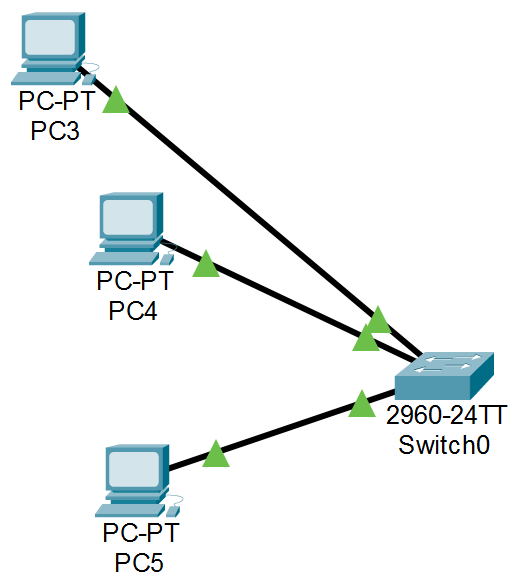
\includegraphics[width=12cm, height=8cm]{Q3-s1.png}
  \caption{LAN-B topology: Three PCs (PC3, PC4, PC5) connected to a Cisco 2960-24TT switch (Switch0).}
  \label{fig:q3_topo}
\end{figure}

\subsection{Before Ping: ARP Table and MAC Address Table}
Before any communication occurs, the ARP tables on the hosts and the MAC forwarding table on the switch are empty.

\begin{figure}[H]
  \centering
  \begin{subfigure}[b]{0.96\textwidth}
    \centering
    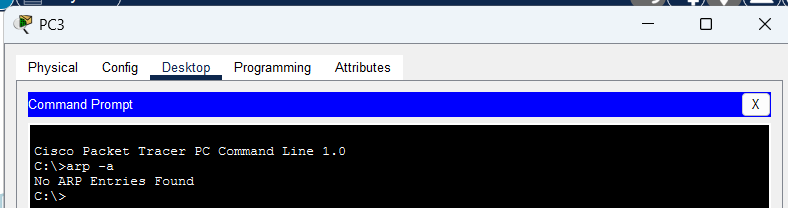
\includegraphics[width=17cm, height=5cm]{Q3-s2.png}
    \caption{PC3: \texttt{arp -a} shows ``No ARP Entries Found'' before any ping.}
    \label{fig:q3_arp_before}
  \end{subfigure}
\end{figure}
\begin{figure}[H]
  \centering
  \begin{subfigure}[b]{0.96\textwidth}
    \centering
    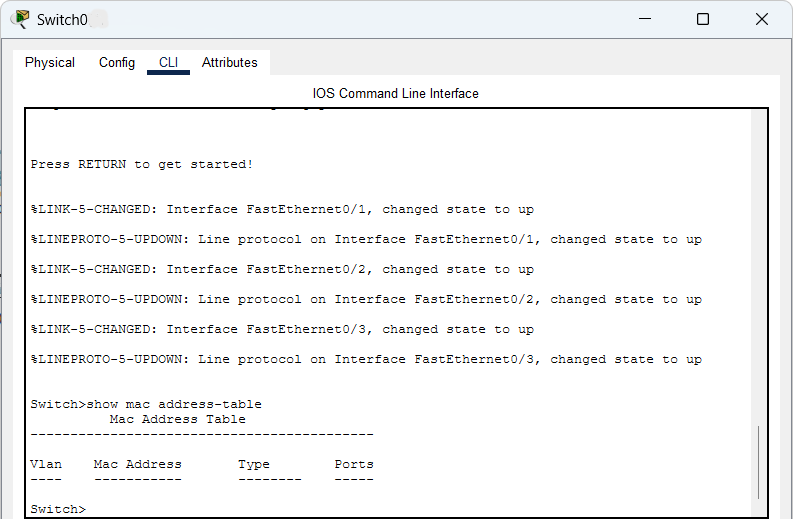
\includegraphics[width=17cm, height=11cm]{Q3-s3.png}
    \caption{Switch0: \texttt{show mac address-table} displays an empty MAC table before any traffic.}
    \label{fig:q3_mac_before}
  \end{subfigure}
  \caption{Empty ARP and MAC address tables before any network communication.}
  \label{fig:q3_before}
\end{figure}

\subsection{Ping Tests Between All Pairs}
Ping tests were conducted between all three pairs of hosts:

\begin{figure}[H]
  \centering
  \begin{subfigure}[b]{0.96\textwidth}
    \centering
    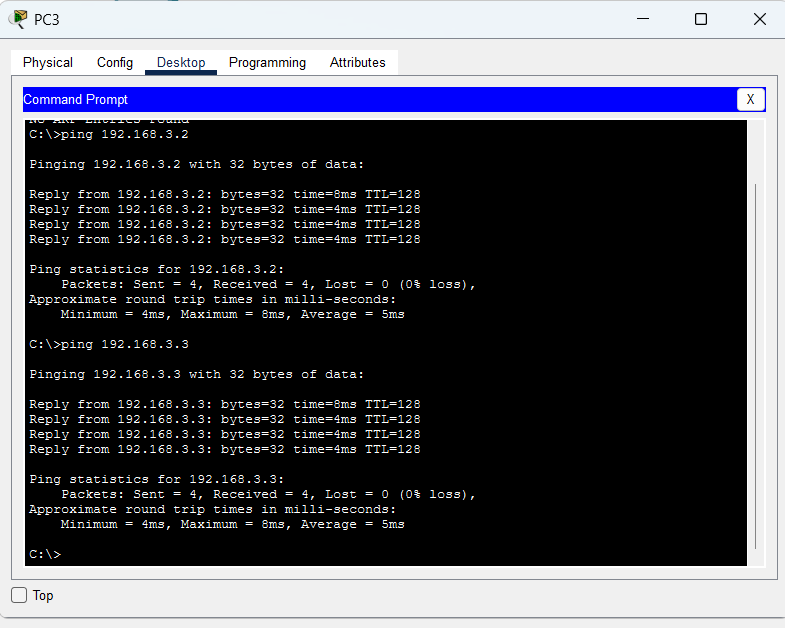
\includegraphics[width=17cm, height=11cm]{Q3-s4.png}
    \caption{PC3 pings PC4 (\texttt{192.168.3.2}) and PC5 (\texttt{192.168.3.3}): all successful.}
    \label{fig:q3_pc3_ping}
  \end{subfigure}
\end{figure}
\begin{figure}[H]
  \centering
  \begin{subfigure}[b]{0.96\textwidth}
    \centering
    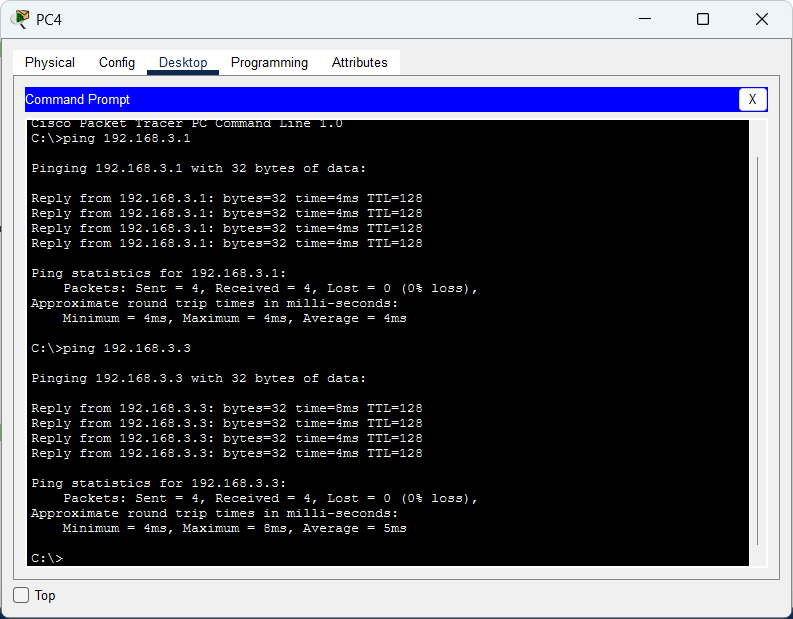
\includegraphics[width=17cm, height=11.5cm]{Q3-s5.png}
    \caption{PC4 pings PC3 (\texttt{192.168.3.1}) and PC5 (\texttt{192.168.3.3}): all successful.}
    \label{fig:q3_pc4_ping}
  \end{subfigure}
\end{figure}
\begin{figure}[H]
  \centering
  \begin{subfigure}[b]{0.96\textwidth}
    \centering
    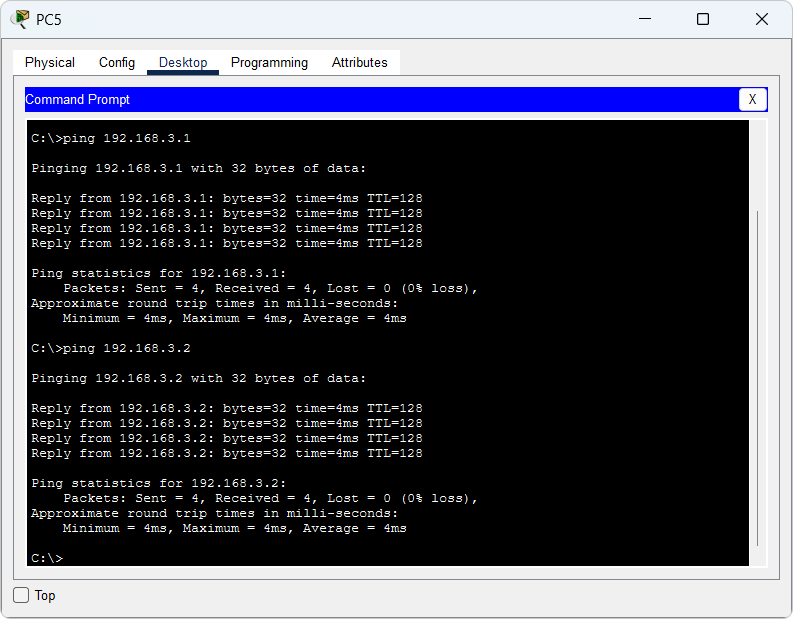
\includegraphics[width=17cm, height=11.5cm]{Q3-s6.png}
    \caption{PC5 pings PC3 (\texttt{192.168.3.1}) and PC4 (\texttt{192.168.3.2}): all successful.}
    \label{fig:q3_pc5_ping}
  \end{subfigure}
  \caption{Ping results between all three pairs of hosts in LAN-B.}
  \label{fig:q3_pings}
\end{figure}

\subsection{After Ping: ARP Table and MAC Address Table}
After the ping exchanges, both the host ARP caches and the switch's MAC address table have been dynamically populated.

\begin{figure}[H]
  \centering
  \begin{subfigure}[b]{0.96\textwidth}
    \centering
    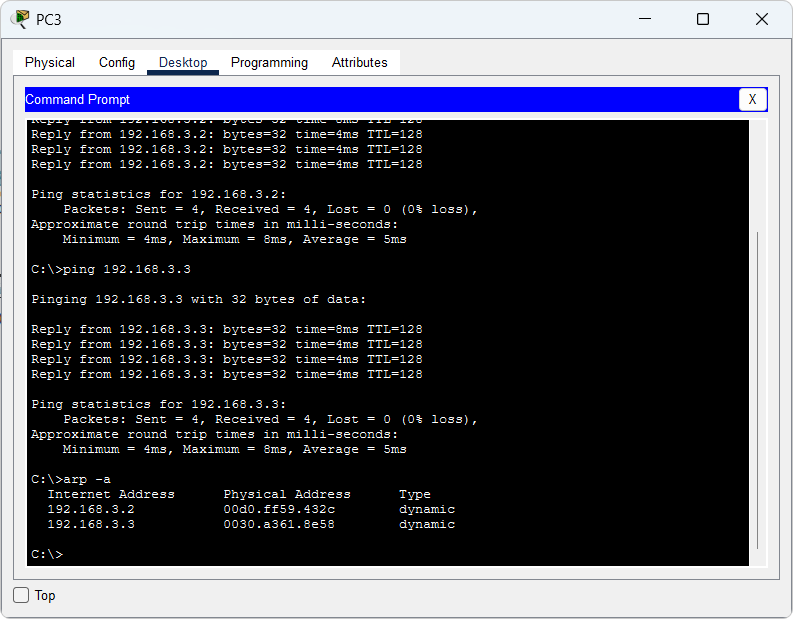
\includegraphics[width=17cm, height=11cm]{Q3-s7.png}
    \caption{PC3: \texttt{arp -a} now shows learned MAC-to-IP mappings for PC4 and PC5.}
    \label{fig:q3_arp_after}
  \end{subfigure}
\end{figure}
\begin{figure}[H]
  \centering
  \begin{subfigure}[b]{0.96\textwidth}
    \centering
    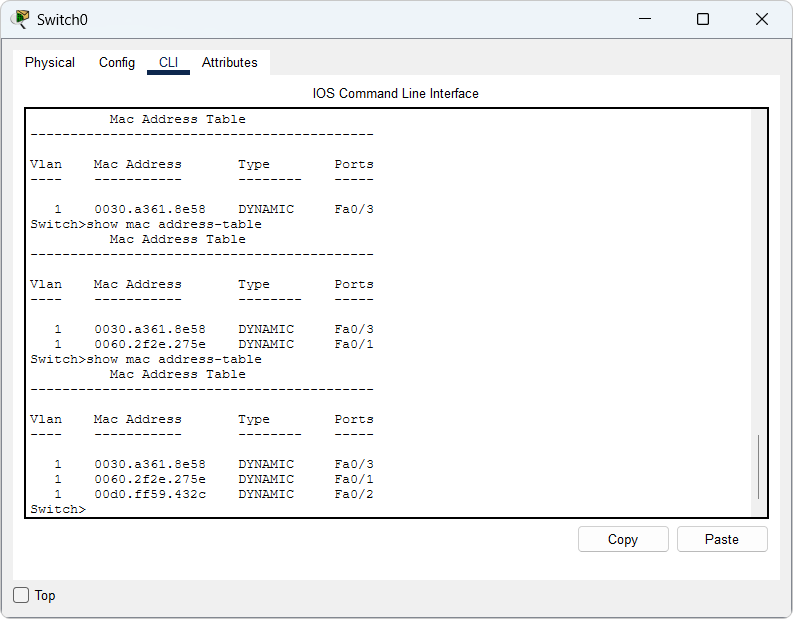
\includegraphics[width=17cm, height=10cm]{Q3-s8.png}
    \caption{Switch0: MAC address table now contains entries for all three connected hosts on their respective ports.}
    \label{fig:q3_mac_after}
  \end{subfigure}
  \caption{Populated ARP and MAC address tables after ping exchanges.}
  \label{fig:q3_after}
\end{figure}

\subsubsection{ARP Table of PC3 (After Pinging)}
\begin{table}[H]
  \centering
  \begin{tabular}{lll}
    \toprule
    \textbf{Internet Address} & \textbf{Physical Address} & \textbf{Type} \\
    \midrule
    \texttt{192.168.3.2} & \texttt{00d0.ff59.432c} & dynamic \\
    \texttt{192.168.3.3} & \texttt{0030.a361.8e58} & dynamic \\
    \bottomrule
  \end{tabular}
  \caption{ARP table of PC3 after pinging PC4 and PC5.}
  \label{tab:q3_arp}
\end{table}

\subsubsection{MAC Address Table of Switch0 (After Pinging)}
The switch MAC address table was observed at three progressive stages using \texttt{show mac address-table}:
\begin{table}[H]
  \centering
  \begin{tabular}{cllll}
    \toprule
    \textbf{Stage} & \textbf{VLAN} & \textbf{MAC Address} & \textbf{Type} & \textbf{Port} \\
    \midrule
    After 1st ping  & 1 & \texttt{0030.a361.8e58} & DYNAMIC & Fa0/3 \\
    \midrule
    After 2nd ping  & 1 & \texttt{0030.a361.8e58} & DYNAMIC & Fa0/3 \\
                     & 1 & \texttt{0060.2f2e.275e} & DYNAMIC & Fa0/1 \\
    \midrule
    After all pings  & 1 & \texttt{0030.a361.8e58} & DYNAMIC & Fa0/3 \\
                     & 1 & \texttt{0060.2f2e.275e} & DYNAMIC & Fa0/1 \\
                     & 1 & \texttt{00d0.ff59.432c} & DYNAMIC & Fa0/2 \\
    \bottomrule
  \end{tabular}
  \caption{Progressive MAC address table learning on Switch0.}
  \label{tab:q3_mac}
\end{table}

\noindent \textbf{Key Observation:} The switch dynamically \textit{learns} MAC addresses by examining the source MAC address field of incoming Ethernet frames and associates each address with the port on which the frame arrived. This is the fundamental operation of a Layer-2 switch, enabling it to forward frames intelligently rather than broadcasting them to all ports like a hub.

% =========================================================================
% SECTION 5: QUESTION 4 - CONNECTING LAN-A AND LAN-B
% =========================================================================
\section{Question 4: Connecting LAN-A and LAN-B via Crossover Cable}

\subsection{Problem Statement}
\begin{quote}
\small\textit{Connect LAN-A and LAN-B by connecting the hub and switch using a crossover cable. Ping between each pair of hosts of LAN-A and LAN-B. Now record the contents of the ARP Table of end hosts and the MAC Forwarding Table of the switch again.}
\end{quote}

\subsection{Experimental Setup}
LAN-A (hub-based, 192.168.2.0/24 subnet) and LAN-B (switch-based, originally 192.168.3.0/24) were reconfigured onto the \textbf{same subnet} (\texttt{192.168.2.0/24}) so that all six hosts could communicate at Layer 2. The hub (Hub1) and switch (Switch2) were interconnected using a \textbf{crossover cable}.

\begin{figure}[H]
  \centering
  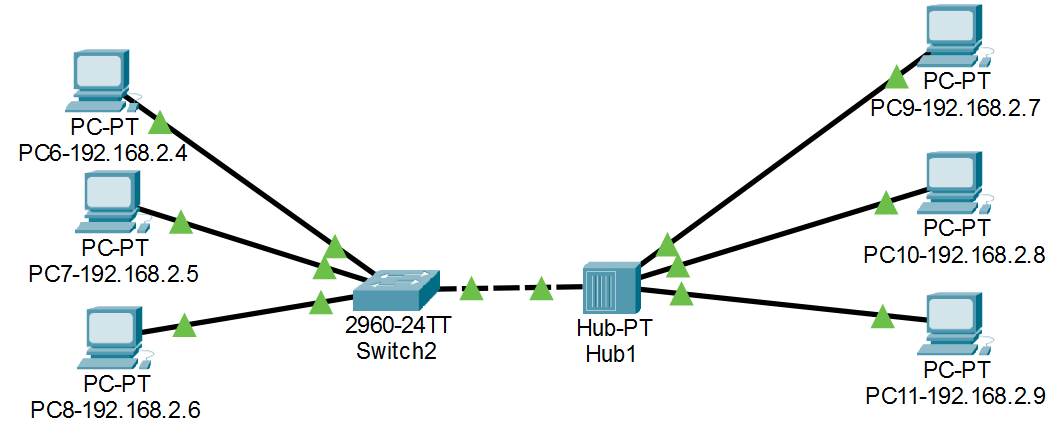
\includegraphics[width=1.0\textwidth]{Q4-s1.png}
  \caption{Combined topology: LAN-B hosts (PC6, PC7, PC8 on Switch2) connected to LAN-A hosts (PC9, PC10, PC11 on Hub1) via a crossover cable between the switch and hub. All hosts are on subnet \texttt{192.168.2.0/24}.}
  \label{fig:q4_topo}
\end{figure}

\subsubsection{IP Address Configuration}
\begin{table}[H]
  \centering
  \begin{tabular}{lccl}
    \toprule
    \textbf{Host} & \textbf{IP Address} & \textbf{Subnet Mask} & \textbf{Connected To} \\
    \midrule
    PC6  & \texttt{192.168.2.4} & \texttt{255.255.255.0} & Switch2 (LAN-B) \\
    PC7  & \texttt{192.168.2.5} & \texttt{255.255.255.0} & Switch2 (LAN-B) \\
    PC8  & \texttt{192.168.2.6} & \texttt{255.255.255.0} & Switch2 (LAN-B) \\
    PC9  & \texttt{192.168.2.7} & \texttt{255.255.255.0} & Hub1 (LAN-A) \\
    PC10 & \texttt{192.168.2.8} & \texttt{255.255.255.0} & Hub1 (LAN-A) \\
    PC11 & \texttt{192.168.2.9} & \texttt{255.255.255.0} & Hub1 (LAN-A) \\
    \bottomrule
  \end{tabular}
  \caption{IP address assignment for the combined LAN-A and LAN-B network.}
  \label{tab:q4_ip}
\end{table}

\subsection{Cross-LAN Ping Tests and ARP/MAC Tables}

\begin{figure}[H]
  \centering
  \begin{subfigure}[b]{0.96\textwidth}
    \centering
    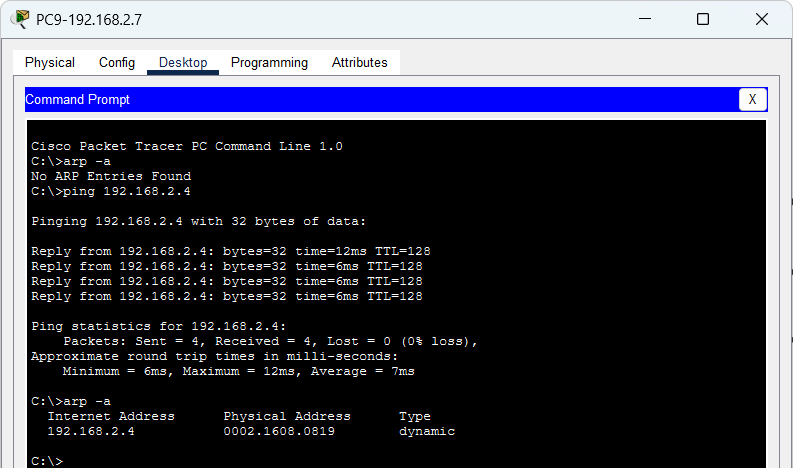
\includegraphics[width=17cm, height=8cm]{Q4-s2.png}
    \caption{PC9 (Hub side, \texttt{192.168.2.7}) pings PC6 (Switch side, \texttt{192.168.2.4}): successful with ARP table showing the learned MAC address.}
    \label{fig:q4_ping}
  \end{subfigure}
\end{figure}
\begin{figure}[H]
  \centering
  \begin{subfigure}[b]{0.96\textwidth}
    \centering
    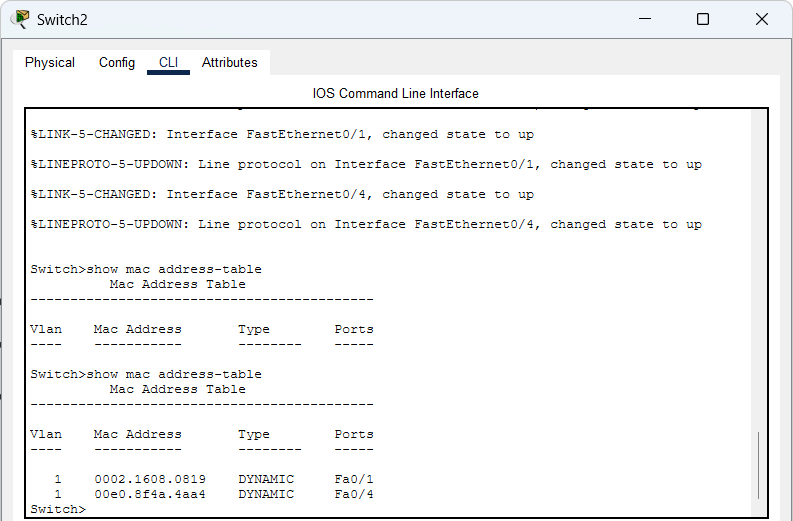
\includegraphics[width=17cm, height=8cm]{Q4-s3.png}
    \caption{Switch2 MAC address table after cross-LAN pings: entries learned on Fa0/1 (from hub via crossover) and Fa0/4 (directly connected host).}
    \label{fig:q4_mac}
  \end{subfigure}
  \caption{Cross-LAN connectivity verification and switch MAC address table state.}
  \label{fig:q4_results}
\end{figure}

\subsubsection{ARP Table of PC9 (After Cross-LAN Ping)}
\begin{table}[H]
  \centering
  \begin{tabular}{lll}
    \toprule
    \textbf{Internet Address} & \textbf{Physical Address} & \textbf{Type} \\
    \midrule
    \texttt{192.168.2.4} & \texttt{0002.1608.0819} & dynamic \\
    \bottomrule
  \end{tabular}
  \caption{ARP table of PC9 after pinging PC6 across the hub-switch bridge.}
  \label{tab:q4_arp}
\end{table}

\subsubsection{MAC Address Table of Switch2 (After Cross-LAN Pings)}
\begin{table}[H]
  \centering
  \begin{tabular}{cllll}
    \toprule
    \textbf{VLAN} & \textbf{MAC Address} & \textbf{Type} & \textbf{Port} & \textbf{Origin} \\
    \midrule
    1 & \texttt{0002.1608.0819} & DYNAMIC & Fa0/1 & PC6 (via switch port) \\
    1 & \texttt{00e0.8f4a.4aa4} & DYNAMIC & Fa0/4 & PC9 (via hub crossover link) \\
    \bottomrule
  \end{tabular}
  \caption{Switch2 MAC address table after cross-LAN communication.}
  \label{tab:q4_mac}
\end{table}

\noindent \textbf{Key Observation:} When the hub and switch are connected via a crossover cable and all hosts are on the same subnet, communication is possible across both LAN segments at Layer 2. The switch learns the MAC addresses of hub-side hosts through the crossover link port (Fa0/4), while the hub simply broadcasts all frames received from the switch to all its connected hosts.

% =========================================================================
% SECTION 6: QUESTION 5 - INTER-LAN ROUTING
% =========================================================================
\section{Question 5: Inter-LAN Routing with Static Routes}

\subsection{Problem Statement}
\begin{quote}
\small\textit{Create a LAN (named JU-Main) with three hosts connected via a layer-2 switch (Cisco 2950 switch). Connect the switch to a router (Cisco 1841). Assign IP addresses from network 192.168.148.0/24. Create another LAN (named JU-SL) with three hosts connected via another switch and router. Assign IP addresses from network 192.168.149.0/24. Connect the two routers through WAN interfaces from network 192.168.150.0/24. Add static routes in both routers to route packets between two LANs.}
\end{quote}

\subsection{Network Topology}
\begin{figure}[H]
  \centering
  \makebox[\textwidth][c]{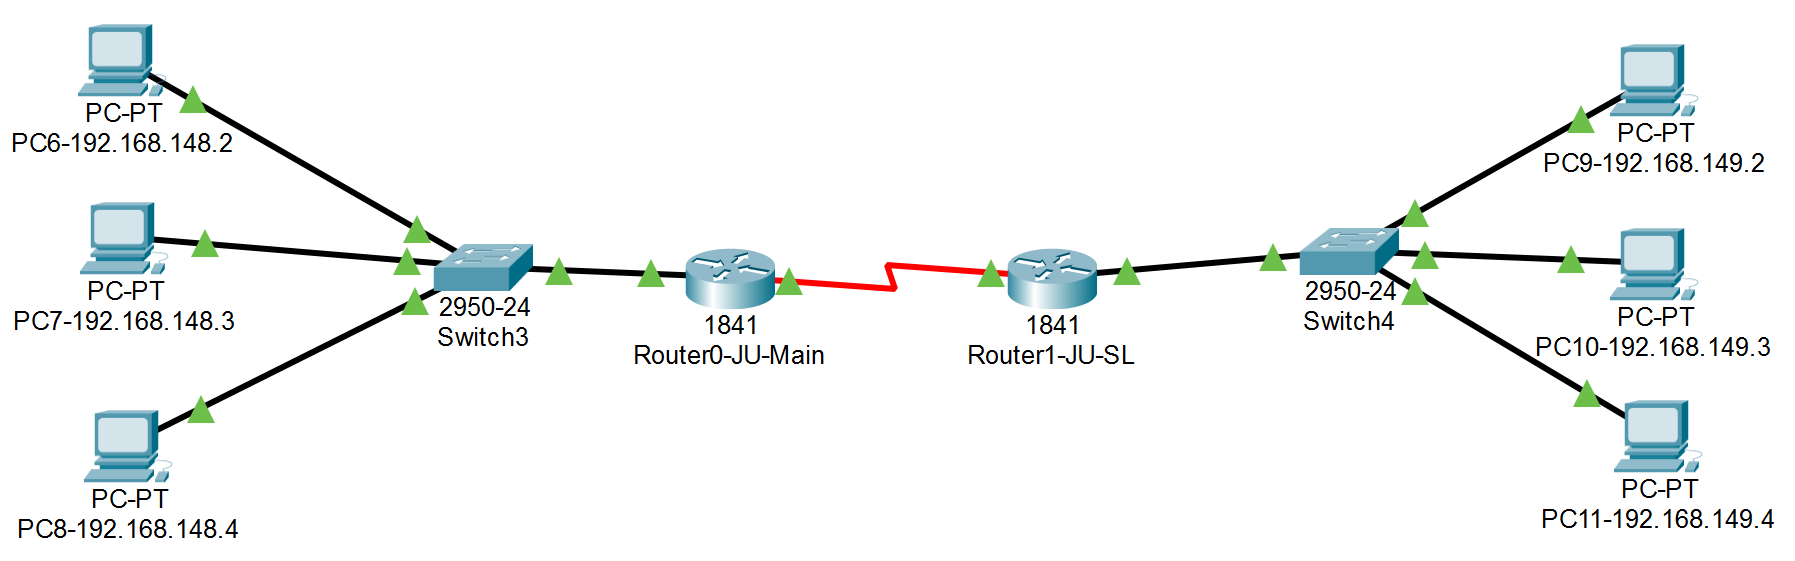
\includegraphics[width=1.15\textwidth, height=8cm]{Q5-s1.png}}
  \caption{Complete internetwork topology: JU-Main LAN (left) and JU-SL LAN (right) interconnected via two Cisco 1841 routers (Router0-JU-Main and Router1-JU-SL) through a Serial WAN link.}
  \label{fig:q5_topo}
\end{figure}

\subsubsection{IP Address Configuration}
\begin{table}[H]
  \centering
  \footnotesize
  \begin{tabularx}{\textwidth}{llccX}
    \toprule
    \textbf{Network} & \textbf{Device} & \textbf{IP Address} & \textbf{Subnet Mask} & \textbf{Role} \\
    \midrule
    \multirow{4}{*}{JU-Main (192.168.148.0/24)} & Router0 Fa0/0 & 192.168.148.1 & 255.255.255.0 & Default Gateway \\
     & PC6 & 192.168.148.2 & 255.255.255.0 & End Host \\
     & PC7 & 192.168.148.3 & 255.255.255.0 & End Host \\
     & PC8 & 192.168.148.4 & 255.255.255.0 & End Host \\
    \midrule
    \multirow{4}{*}{JU-SL (192.168.149.0/24)} & Router1 Fa0/0 & 192.168.149.1 & 255.255.255.0 & Default Gateway \\
     & PC9 & 192.168.149.2 & 255.255.255.0 & End Host \\
     & PC10 & 192.168.149.3 & 255.255.255.0 & End Host \\
     & PC11 & 192.168.149.4 & 255.255.255.0 & End Host \\
    \midrule
    \multirow{2}{*}{WAN Link (192.168.150.0/24)} & Router0 Serial0/0/0 & 192.168.150.1 & 255.255.255.0 & DCE/DTE \\
     & Router1 Serial0/0/0 & 192.168.150.2 & 255.255.255.0 & DCE/DTE \\
    \bottomrule
  \end{tabularx}
  \caption{Complete IP addressing scheme for the JU-Main and JU-SL internetwork.}
  \label{tab:q5_ip}
\end{table}

\subsection{Router Configuration and Static Routes}
Static routes were configured on both routers to enable inter-LAN communication:

\begin{figure}[H]
  \centering
  \begin{subfigure}[b]{0.96\textwidth}
    \centering
    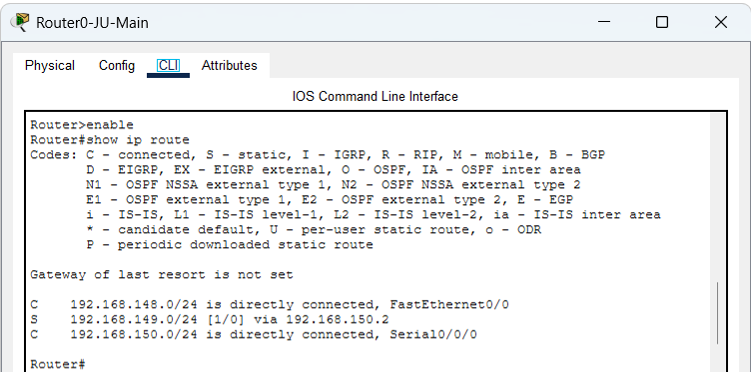
\includegraphics[width=17cm, height=6cm]{Q5-s2.png}
    \caption{Router0 (JU-Main): Routing table showing connected routes (C) for \texttt{192.168.148.0/24} and \texttt{192.168.150.0/24}, and a static route (S) to \texttt{192.168.149.0/24} via \texttt{192.168.150.2}.}
    \label{fig:q5_r0}
  \end{subfigure}
\end{figure}
\begin{figure}[H]
  \centering
  \begin{subfigure}[b]{0.96\textwidth}
    \centering
    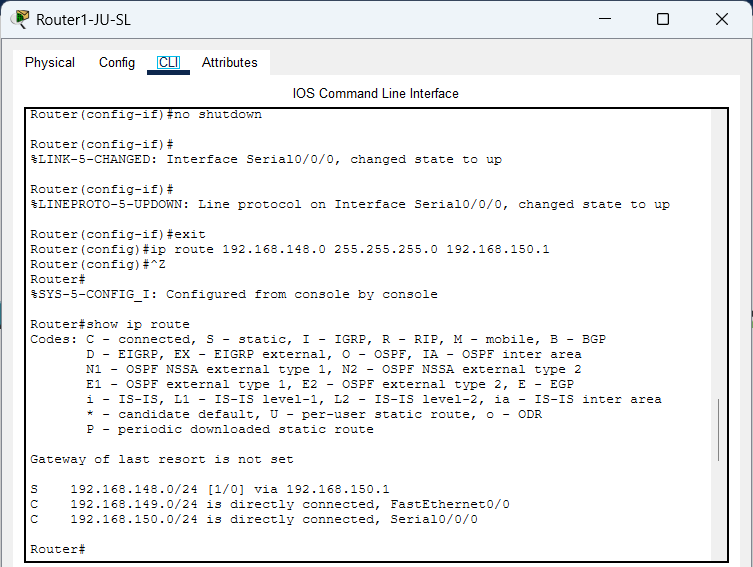
\includegraphics[width=17cm, height=8.5cm]{Q5-s3.png}
    \caption{Router1 (JU-SL): Routing table showing connected routes (C) for \texttt{192.168.149.0/24} and \texttt{192.168.150.0/24}, and a static route (S) to \texttt{192.168.148.0/24} via \texttt{192.168.150.1}.}
    \label{fig:q5_r1}
  \end{subfigure}
  \caption{Routing tables of both routers confirming static route configuration.}
  \label{fig:q5_routes}
\end{figure}

\subsubsection{Static Route Commands}
\begin{lstlisting}[style=cmdstyle]
! Router0-JU-Main:
Router(config)#ip route 192.168.149.0 255.255.255.0 192.168.150.2

! Router1-JU-SL:
Router(config)#ip route 192.168.148.0 255.255.255.0 192.168.150.1
\end{lstlisting}

\subsection{Inter-LAN Ping Verification}
\begin{figure}[H]
  \centering
  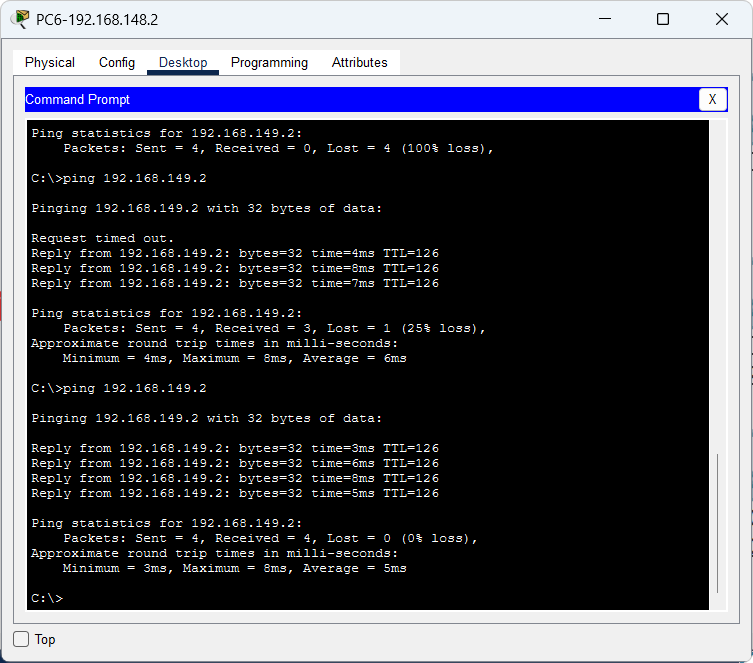
\includegraphics[width=\textwidth, height=12cm]{Q5-s4.png}
  \caption{PC6 (\texttt{192.168.148.2}) in JU-Main pinging PC9 (\texttt{192.168.149.2}) in JU-SL: initial request times out (ARP resolution), subsequent packets successful with TTL=126 (two router hops). Second ping attempt shows 0\% loss.}
  \label{fig:q5_ping}
\end{figure}

\noindent \textbf{Key Observations:}
\begin{itemize}
  \item The first ping attempt had 25\% packet loss (1 timeout) because the initial ARP resolution across routers introduces additional delay.
  \item The TTL value of \textbf{126} (instead of the default 128) confirms that the ICMP packet traversed \textbf{two router hops}: Router0 $\rightarrow$ WAN link $\rightarrow$ Router1.
  \item The second ping attempt succeeded with 0\% loss, confirming that the static routes are properly configured and operational.
  \item Each host's default gateway must be set to the local router's interface IP address for inter-LAN routing to function correctly.
\end{itemize}

% =========================================================================
% SECTION 7: QUESTION 6 - DHCP CONFIGURATION
% =========================================================================
\section{Question 6: DHCP Server Configuration}

\subsection{Problem Statement}
\begin{quote}
\small\textit{Add servers to the individual LANs (in problem 5) and configure them as a DHCP server. Configure the hosts in the individual LAN to obtain IP addresses and address of the default gateway via this DHCP server.}
\end{quote}

\subsection{Network Topology with DHCP Servers}
\begin{figure}[H]
  \centering
  \makebox[\textwidth][c]{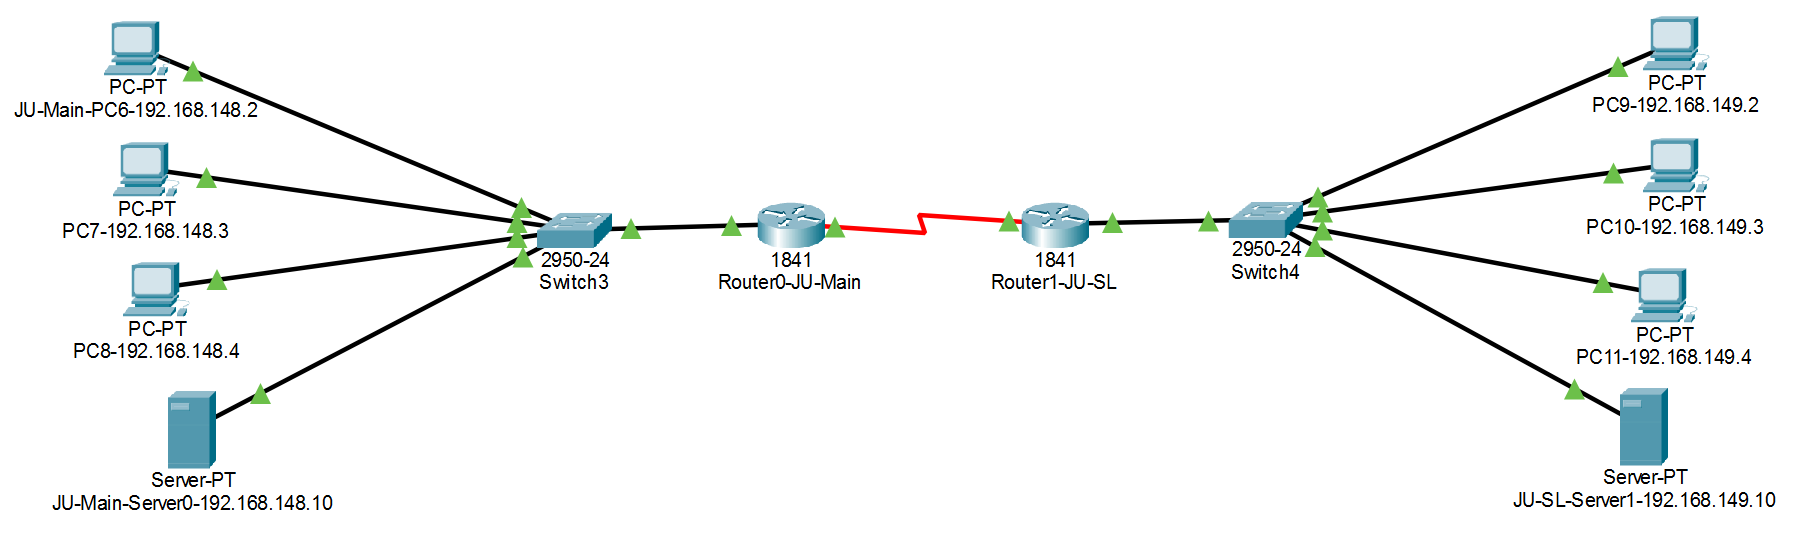
\includegraphics[width=1.15\textwidth, height=6cm]{Q6-s1.png}}
  \caption{Extended topology from Question 5 with DHCP servers added: JU-Main-Server0 (\texttt{192.168.148.10}) on the left and JU-SL-Server1 (\texttt{192.168.149.10}) on the right.}
  \label{fig:q6_topo}
\end{figure}

\subsection{DHCP Server Configuration}
Each server was configured with the DHCP service to dynamically assign IP addresses to hosts on its respective LAN.

\begin{figure}[H]
  \centering
  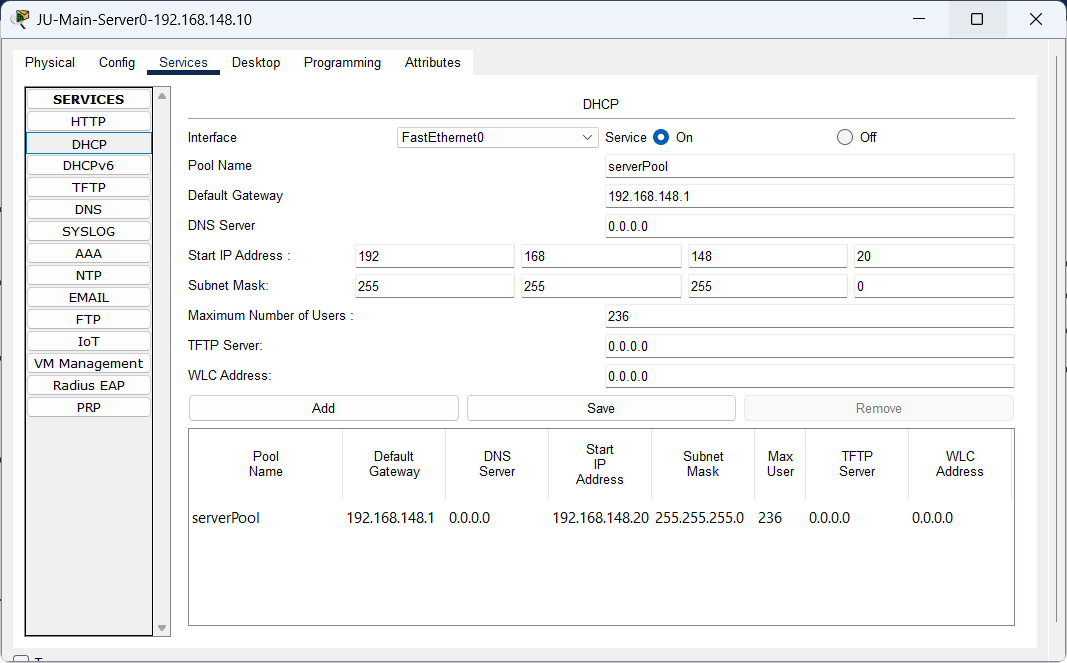
\includegraphics[width=0.85\textwidth]{Q6-s2.png}
  \caption{DHCP configuration on JU-Main-Server0: Pool name ``serverPool'', Default Gateway \texttt{192.168.148.1}, Start IP Address \texttt{192.168.148.20}, Subnet Mask \texttt{255.255.255.0}, Maximum 236 users.}
  \label{fig:q6_dhcp}
\end{figure}

\subsubsection{DHCP Pool Parameters}
\begin{table}[H]
  \centering
  \footnotesize
  \begin{tabularx}{\textwidth}{lccccX}
    \toprule
    \textbf{Server} & \textbf{Pool Name} & \textbf{Gateway} & \textbf{Start IP} & \textbf{Subnet Mask} & \textbf{Max Users} \\
    \midrule
    JU-Main-Server0 & serverPool & 192.168.148.1 & 192.168.148.20 & 255.255.255.0 & 236 \\
    JU-SL-Server1   & serverPool & 192.168.149.1 & 192.168.149.20 & 255.255.255.0 & 236 \\
    \bottomrule
  \end{tabularx}
  \caption{DHCP pool configuration for both LAN servers.}
  \label{tab:q6_dhcp}
\end{table}

\subsection{DHCP Client Verification}
Hosts were reconfigured from static to DHCP addressing mode. Upon enabling DHCP, each host broadcasts a DHCP Discover message, receives a DHCP Offer from the server, requests the offered address (DHCP Request), and receives confirmation (DHCP Acknowledge).

\begin{figure}[H]
  \centering
  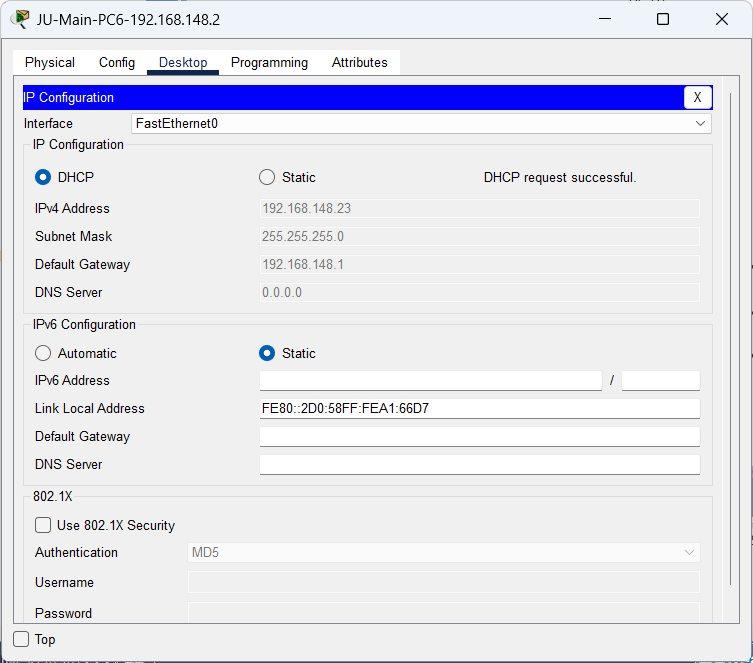
\includegraphics[width=17cm, height=15cm]{Q6-s3.png}
  \caption{JU-Main-PC6 IP Configuration showing ``DHCP request successful'': dynamically assigned IP \texttt{192.168.148.23}, Subnet Mask \texttt{255.255.255.0}, Default Gateway \texttt{192.168.148.1}.}
  \label{fig:q6_client}
\end{figure}

\noindent \textbf{Key Observations:}
\begin{itemize}
  \item The DHCP server automatically assigned IP address \texttt{192.168.148.23} to PC6, starting from the configured pool start address (\texttt{192.168.148.20}).
  \item The default gateway (\texttt{192.168.148.1}) was automatically provided to the client, eliminating manual gateway configuration.
  \item The DHCP process follows the standard \textbf{DORA} sequence: \textbf{D}iscover $\rightarrow$ \textbf{O}ffer $\rightarrow$ \textbf{R}equest $\rightarrow$ \textbf{A}cknowledge.
\end{itemize}

% =========================================================================
% SECTION 8: QUESTION 7 - DNS, WEB, FTP, DHCP LAN
% =========================================================================
\section{Question 7: Complete LAN with DNS, Web, FTP, and DHCP Servers}

\subsection{Problem Statement}
\begin{quote}
\small\textit{Create a LAN (CSE) with three hosts connected via a layer-2 switch (Cisco 2950 switch CSE-Switch). Also add a web server and an FTP server to this LAN. The hosts dynamically get their IP addresses from a local DHCP server. Servers are assigned fixed IP addresses. Add a Domain Name Server (DNS) to this LAN. Create appropriate records in the DNS server for the individual servers in the LAN. The domain name of the LAN is cse.myuniv.edu. Configure the individual hosts to use the local DNS server for name resolution.}
\end{quote}

\subsection{Network Topology}
\begin{figure}[H]
  \centering
  \makebox[\textwidth][c]{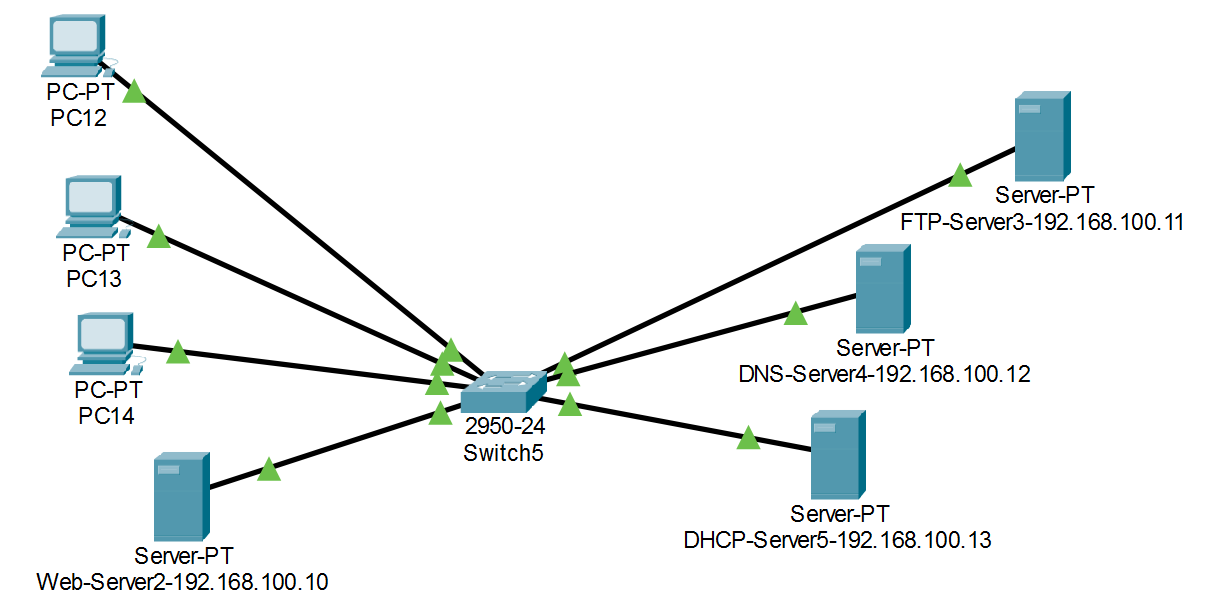
\includegraphics[width=1.10\textwidth', height=8cm]{Q7-s1.png}}
  \caption{CSE LAN topology: Three hosts (PC12, PC13, PC14) and four servers (Web-Server2, FTP-Server3, DNS-Server4, DHCP-Server5) connected via Cisco 2950-24 Switch5.}
  \label{fig:q7_topo}
\end{figure}

\subsubsection{Server IP Address Configuration}
\begin{table}[H]
  \centering
  \begin{tabular}{lccl}
    \toprule
    \textbf{Server} & \textbf{IP Address} & \textbf{Subnet Mask} & \textbf{Service} \\
    \midrule
    Web-Server2    & \texttt{192.168.100.10} & \texttt{255.255.255.0} & HTTP \\
    FTP-Server3    & \texttt{192.168.100.11} & \texttt{255.255.255.0} & FTP \\
    DNS-Server4    & \texttt{192.168.100.12} & \texttt{255.255.255.0} & DNS \\
    DHCP-Server5   & \texttt{192.168.100.13} & \texttt{255.255.255.0} & DHCP \\
    \bottomrule
  \end{tabular}
  \caption{Static IP address assignment for all servers in the CSE LAN.}
  \label{tab:q7_servers}
\end{table}

\subsection{DNS Server Configuration}
The DNS server was configured with A records mapping domain names to server IP addresses within the \texttt{cse.myuniv.edu} domain:

\begin{figure}[H]
  \centering
  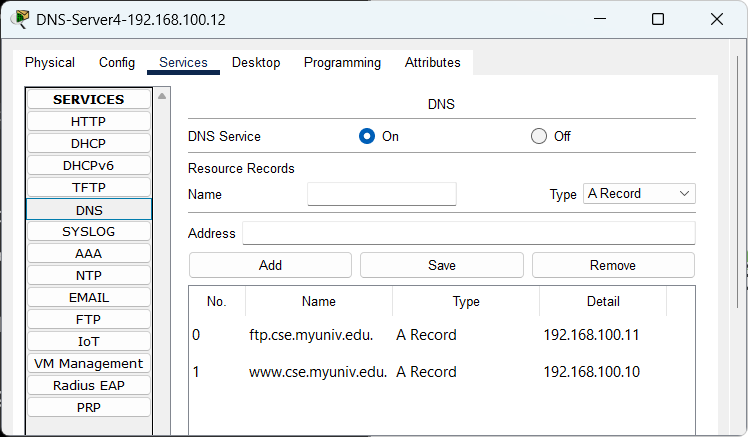
\includegraphics[width=0.75\textwidth]{Q7-s2.png}
  \caption{DNS-Server4 configuration showing two A records: \texttt{ftp.cse.myuniv.edu.} $\rightarrow$ \texttt{192.168.100.11} and \texttt{www.cse.myuniv.edu.} $\rightarrow$ \texttt{192.168.100.10}.}
  \label{fig:q7_dns}
\end{figure}

\subsubsection{DNS Resource Records}
\begin{table}[H]
  \centering
  \begin{tabular}{clll}
    \toprule
    \textbf{No.} & \textbf{Name (FQDN)} & \textbf{Type} & \textbf{Detail (IP Address)} \\
    \midrule
    0 & \texttt{ftp.cse.myuniv.edu.} & A Record & \texttt{192.168.100.11} \\
    1 & \texttt{www.cse.myuniv.edu.} & A Record & \texttt{192.168.100.10} \\
    \bottomrule
  \end{tabular}
  \caption{DNS A Records configured on DNS-Server4 for the \texttt{cse.myuniv.edu} domain.}
  \label{tab:q7_dns}
\end{table}

\subsection{Web Server Access via DNS}
With DNS properly configured, hosts can access the web server using its domain name rather than its IP address.

\begin{figure}[H]
  \centering
  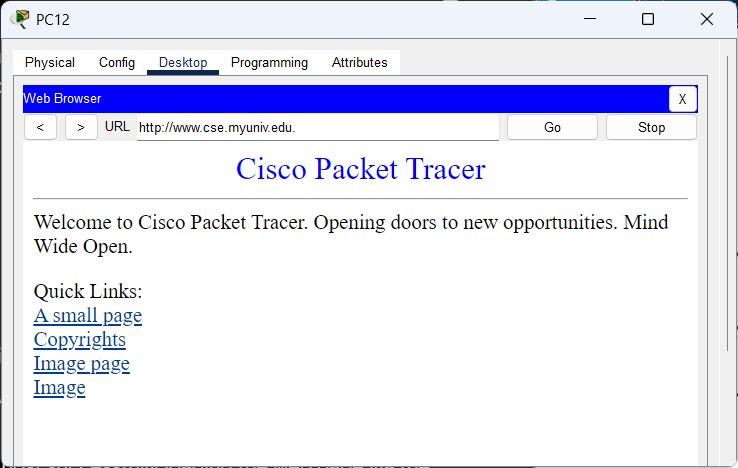
\includegraphics[width=0.65\textwidth]{Q7-s3.png}
  \caption{PC12 accessing the web server via URL \texttt{http://www.cse.myuniv.edu.}: the DNS server resolves the domain name to \texttt{192.168.100.10}, and the Cisco Packet Tracer default web page is displayed.}
  \label{fig:q7_web}
\end{figure}

\subsection{FTP Server Access via DNS}
The FTP server was also accessed using its DNS-resolved domain name:

\begin{figure}[H]
  \centering
  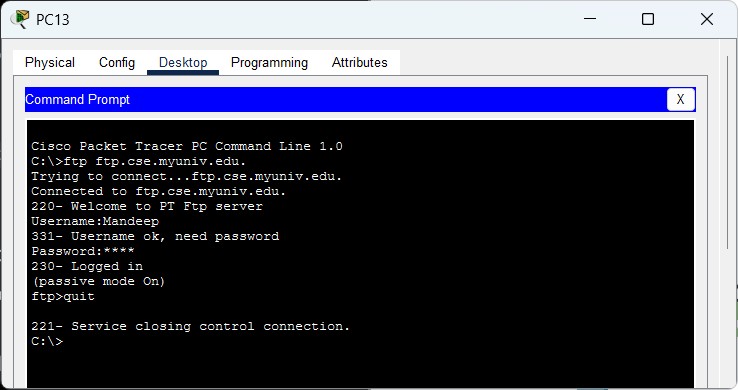
\includegraphics[width=17cm, height=10cm]{Q7-s4.png}
  \caption{PC13 connecting to the FTP server via \texttt{ftp ftp.cse.myuniv.edu.}: the DNS server resolves the domain name, user ``Mandeep'' authenticates successfully, and the session is established.}
  \label{fig:q7_ftp}
\end{figure}

\noindent As shown in Figure \ref{fig:q7_ftp}, the FTP session proceeds through the following steps:
\begin{enumerate}
  \item DNS resolution: \texttt{ftp.cse.myuniv.edu.} $\rightarrow$ \texttt{192.168.100.11}
  \item TCP connection established to port 21
  \item Server banner: \texttt{220- Welcome to PT FTP server}
  \item User authentication: Username ``Mandeep'' with password $\rightarrow$ \texttt{230- Logged in}
  \item Passive mode enabled, session operational
  \item Clean disconnection via \texttt{quit} $\rightarrow$ \texttt{221- Service closing control connection}
\end{enumerate}

\noindent \textbf{Key Observations:}
\begin{itemize}
  \item The DHCP server dynamically assigns IP addresses and DNS server addresses to the three hosts.
  \item The DNS server provides centralized name resolution, allowing hosts to access services by memorable domain names instead of IP addresses.
  \item Both HTTP and FTP services are fully operational and accessible through DNS-resolved FQDNs.
  \item The domain structure follows the convention: \texttt{service.cse.myuniv.edu}, where \texttt{service} is either \texttt{www} or \texttt{ftp}.
\end{itemize}

% =========================================================================
% SECTION 9: CONCLUSION
% =========================================================================
\section{Conclusion and Comments}

\subsection{Summary of Results}
This laboratory assignment successfully demonstrated progressively complex network configurations using Cisco Packet Tracer. Key findings across all seven experiments include:
\begin{enumerate}
  \item \textbf{Direct Connectivity:} Two PCs connected via a crossover cable can communicate directly without any intermediate networking device, provided they are on the same IP subnet.
  \item \textbf{Hub-based LAN:} A hub creates a single broadcast and collision domain. All connected hosts can communicate, but all traffic is visible to all hosts (no frame filtering).
  \item \textbf{Switch-based LAN:} A switch dynamically learns MAC addresses and builds a forwarding table, enabling intelligent unicast forwarding. Before any traffic, both ARP and MAC tables are empty; after pinging, they are fully populated.
  \item \textbf{Hub-Switch Interconnection:} Hosts on a hub and switch can communicate when connected via a crossover cable on the same subnet. The switch learns hub-side MAC addresses through the interconnection port.
  \item \textbf{Inter-LAN Routing:} Static routes enable communication between hosts on different subnets across router boundaries. The TTL decrement (128 $\rightarrow$ 126) confirms two-hop routing.
  \item \textbf{DHCP Automation:} DHCP servers eliminate manual IP configuration by dynamically assigning addresses, subnet masks, and default gateways to clients via the DORA process.
  \item \textbf{DNS-based Service Access:} DNS servers provide domain-to-IP resolution, enabling user-friendly access to web and FTP services using fully qualified domain names.
\end{enumerate}

\subsection{What I Learned}
\begin{itemize}
  \item Understood the operational differences between Layer-1 hubs (broadcast) and Layer-2 switches (intelligent forwarding).
  \item Gained practical experience in configuring IP addressing, static routing, DHCP, and DNS services.
  \item Observed the relationship between ARP tables (IP-to-MAC mapping) and switch MAC address tables (MAC-to-port mapping).
  \item Learned to configure WAN serial links between routers and establish inter-LAN reachability through static routes.
\end{itemize}

% =========================================================================
% REFERENCES
% =========================================================================
\subsection{References Used}
\begin{itemize}
  \item Kurose, J. F., and Ross, K. W., \textit{Computer Networking: A Top-Down Approach}, 8th ed., Pearson, 2021.
  \item Cisco Systems, \textit{Cisco Packet Tracer Documentation}, \url{https://www.netacad.com/courses/packet-tracer}, 2026.
  \item IEEE Standards Association, \textit{IEEE Standard for Ethernet}, IEEE Std 802.3-2022.
\end{itemize}

\end{document}
